\documentclass[10pt,
superscriptaddress,
amsmath,amssymb,showkeys,
aps, 
prb,
]{revtex4-2}
\usepackage[T1]{fontenc}
\usepackage{graphicx}% Include figure files
\usepackage{subcaption}

\usepackage{bm}% bold math
\usepackage{physics}
\usepackage{todonotes}
\usepackage{helvet}
\usepackage{color}
\renewcommand{\familydefault}{\sfdefault}

\usepackage[a4paper, margin=0.5cm]{geometry}
\usepackage[export]{adjustbox}
\usepackage{hyperref}
\hypersetup{
	colorlinks=true,
	linkcolor=blue,
	filecolor=magenta,      
	urlcolor=cyan,
	pdfpagemode=FullScreen,
}
\usepackage{autobreak}
\usepackage{bbm}
\usepackage[normalem]{ulem}
\usepackage[absolute,overlay]{textpos}

\newcommand{\response}[1]{{\color{black}#1}} % for authors' response
\newcommand{\comment}[1]{{\color{blue}#1}} % for referee's comment


\begin{document}
\preprint{Preprint}

\title{Response to Referee Comments for Manuscript NJP-117075}
\author{Mahbub Rahaman, Akitada Sakurai, Analabha Roy}
\date{\today}

\maketitle

\vspace{1em}

\noindent \textbf{Response to the Referee: 2's comment}
\begin{enumerate}
	\item {\bf Major Comments}
	\begin{enumerate}
		\item The referee comments on, \comment{``System size dependence: The manuscript presents insightful results for a system size
				of N=8; however, a crucial aspect remains unexplored – the dependence of the
				findings on the system size. How do the observed dynamics and stability vary with an
				increase in system size?"}\\
		
		\response{
			We appreciate the referee's comment. We have expanded our investigation on the establishment and maintenance of quantum chimeralike order for system sizes larger than N=8. The figure (9) displays the regional magnetization ($M^z_A$) plot, which demonstrates melting in the DTC phase. Additionally, there are beats observed at all types of spin interactions (as defined by $\beta$) and coupling strengths in the $M^z_A$ curves in region A. In order to comprehend the melting in DTC observation, we have taken into account sizes from smaller ones to larger ones, such as N = 4, 6, 8, 10 and computed the numerical values of $M^z_A$ at the DTC/DL point. The DTC/DL point corresponds to the first zero of the Bessel function $\mathcal{J}_0\left(\frac{4h}{\omega}\right)$ of the driving parameters, amplitude$(h)$ and frequency $(\omega)$. We then got the associated Fast Fourier Transforms (FFT) for an extended time period of up to $8 \times 10^4$T.   \\		
			
			We have numerically calculated the beat frequency for each case of $\beta$'s from FFT data and spin coupling strengths (weak and strong) and plotted it in figure(12) in the revised manuscript. We've noticed that the frequency of beats decreases as the system size N increases. This demonstrates that the stability of the DTC-DMBL chimeralike order is enhanced as N rises, regardless of the chosen $\beta$ values and coupling strengths. As the number of particles, N, approaches infinity at the thermodynamic limit, the beat frequency disappears, indicating a state of chimeralike order that is entirely stable. We have updated the manuscript to include a part on page no. 19 titled "4.3. System size-dependent stability in chimeralike order," which describes how the stability of chimeralike order depends on the system size.
			
			\begin{figure}[h!]
				\begin{center}
					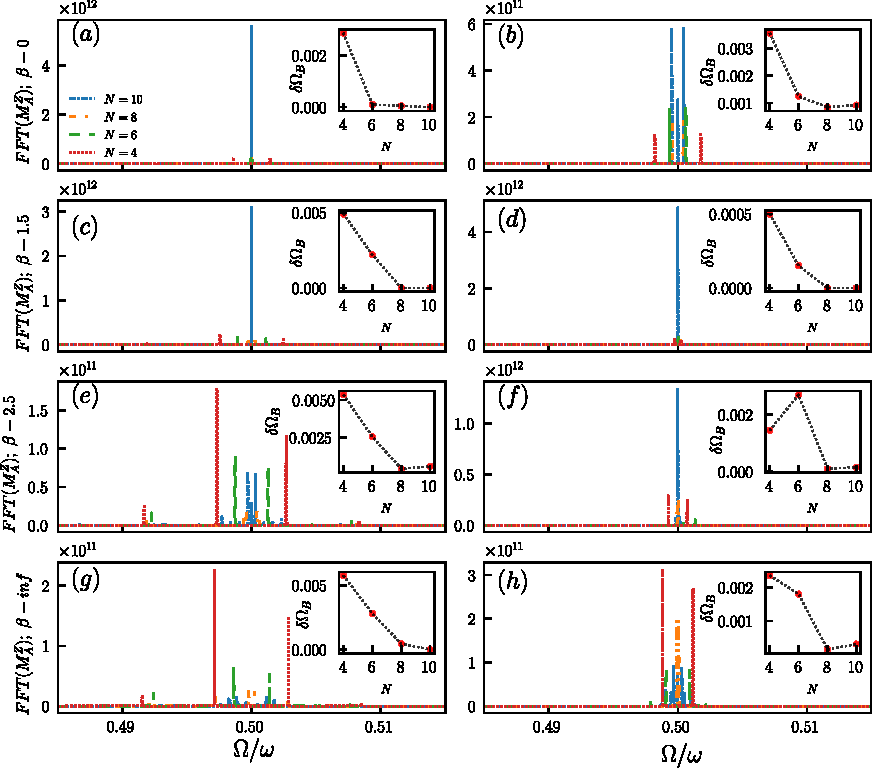
\includegraphics[width=10cm]{./figs/figure12.pdf}
				\end{center}
				\caption{FFT of regional magnetization $M^z_A$ at panels from top to bottom for $8\times10^4$T and spin interaction ranges ($\beta = 0,1.5,2.5, \infty[inf]$). The left and right panels show weak and strong spin coupling. With constant $\omega = 20$ and time period $T= 2\pi/\omega$, the drive parameters are at the CDT/DL point. Each panel's inset shows the beat frequency $\delta\Omega_B$ for various system sizes N.
				}
				\label{Fig:aroundCDT}
			\end{figure}
		}
	
		\item The referee comments on, \comment{``Influence of rotational error $\epsilon_B$: The manuscript effectively investigates the
			impact of $\epsilon_A$={0.03,0.05,0.1} on the chimera states, leaving the role of $\epsilon_B$, set to 0.9, less discussed. How does varying $\epsilon_B$ impact the chimera
			states?"}\\
		
		\response{We appreciate the referee's attention to the matter. We have explored the impact of different rotation errors, specifically $\epsilon_B$, with values of 0.6 and 0.8, while keeping $\epsilon_A$ constant at 0.03. In the revised manuscript, we have included a figure (7) that presents the numerical calculation of the local magnetization $\expval{\hat{S}^z}$ for various $\beta$ values and spin coupling strengths, taking into account the drive parameters at CDT/DL point. It has been observed that the DTC-DMBL order exhibits a lack of stability in course of time in all cases. The stability of the DMBL phase in region B decreases as $\epsilon_B$ increases. The stability of the DTC phase in region A is directly influenced by this. Moreover, we found that, for all-to-all interaction, the local magnetization in region A varies equally. However, for shorter ranges, $\expval{\hat{S}^z}$ decays quickly with a decrease in spin interaction ranges ($\beta >0$) and an increase in the relative distance from the junction between the regions A $\&$ B. We have provided a comprehensive discussion on the matter in section (3), specifically on page 12 to the end of the section.\\
			
		To gain a genreal comprehensive understanding of the stability of the DTC-DMBL chimeralike order, we conducted further research using a wide range of values for $\epsilon_A$ and $\epsilon_B$. We then estimated the regional magnetization $M^z_A$ and $M^z_B$ at the CDT/DL point for certain values of $\beta$ and coupling strengths. The $M^z_{A,B}$ values have been plotted in figure 8 on page 15. We note that the primary factors influencing the stability and selection of DTC and DMBL phases within regions are $\epsilon_A$ and $\epsilon_B$. The DTC-DMBL chimera is most stable when $\epsilon_A$ approaches 0 and $\epsilon_B$ approaches 1.0, representing extreme opposite conditions. When the value of $\epsilon_B$ is less than 0.9 and $\epsilon_A$ is kept constant at 0.03, we see that both regions experience melting of the DTC phase as $\epsilon_B$ decreases gradually. This observation is shown in panels a, b, c, and d. We have also conducted investigations on scenarios where $\epsilon_A\sim\epsilon_B$, and we have observed that these cases do not display the DTC-DMBL chimeralike order. Remarkably, when we hold $\epsilon_B$ constant at 0.1 and increment $\epsilon_A$, we witness an occurrence of DMBL in region A and DTC in region B in the extreme scenario where $\epsilon_A$ is set to 0.1 and $\epsilon_B$ is set to 0.9. We have incorporated this discussion in the revised manuscript in section '4.1. Regional Magnetization' on page 14.
		
		
		}
		\item The referee comments on, \comment{``\underline{Higher root of Bessel function and stability of chimera states:}"}\\
		\begin{enumerate}
			\item \comment{``The paper introduces a higher root of the Bessel function without explicitly justifying its significance. The importance of this higher root and its relevance to the stability
				of chimera states need clarification. How does the selection of a higher root impact the system's behavior, and why is it crucial for the observed dynamics?"}\\
			
			\response{We thank the referee to point out the mistake. To obtain DMBL in $T_2$ cycle, the drive parameters should be considered in a manner that the ratio $\frac{4h}{\omega}$ is one of the roots of Bessel function $\mathcal{J}_0\left(\frac{4h}{\omega}\right)$ which is denoted as `CDT/DL point' as discussed in Appendix-A. There is no restriction on selection over the root of the Bessel function regarding CDT/DL point. We have corrected this issue by defining `CDT/DL point' corresponding to the first root of $\mathcal{J}_0\left(\frac{4h}{\omega}\right)$ at page no,\ref{Put the page number line number etc.} and maintained it through out in the manuscript and updated all the figures in revised manuscript with no change in results with comparison to the earlier manuscript. 
			}
		
			\item \comment{``Moreover, the statement “The stability of the chimera order diminishes even if there is a minor deviation from the CDT/DL point” (page 15, lines 43-44) implies that chimera states might not be stable under slight deviations from the CDT/DL point. This raises a critical question regarding the practical implementation of creating chimera states in experiments. To address this, it would be valuable for the paper to explore potential techniques or strategies aimed at stabilizing the DMBL part of the chain. Elaborating on practical considerations and potential solutions would enhance the paper's applicability and contribute to a more comprehensive understanding of the proposed model."}\\
			
			\response{We thank the referee for the comment. We have considered the drive parameter ratio $\frac{4h}{\omega}$ at fixed to CDT/DL point (which we have chosen to be the first root of the Bessel function for our numerical simulations) which is 2.4048 and the point away from CDT/DL we considered to be 6.0 which is $\sim0.40$ value differ from its closest Bessel function root ($\mathcal{J}_4 =6.3802$). At this point DMBL as well as chimeralike state is unstable. This deviation $~0.40$ is a major deviation from any CDT/DL point. So our claim on instability of chimeralike order at minor deviation in earlier manuscript was incorrect. The minor deviation should be smaller than this regarding the scale of drive parameter ratio. \\
				
			To investigate the stability of chimeralike order around the CDT/DL point we have introduced a minor deviation($\Delta_h$) in range between $\in[-0.05, 0.05]$ to the drive amplitude (h) which corresponds to the CDT/DL point at constant drive frequency $\omega = 20$. We also considered the spins are all up polarized initially and system size to be N=8 and $\beta=0$. One can consider otherwise $\beta$'s; however that would necessitate larger system size which spans larger matrices in product space. We numerically evolve the system for a few time cycles upto 20T and calculate the fidelity ($F_n = \abs{\braket{\psi(0)}{\psi (20T)}}^2$) which measures the closeness of the initial state  to the state of the system at 20T. We have plotted $F_n$ for different $\frac{4\Delta_h}{\omega}$ in figure below. The minor deviation region is filled with gray color. 
			\begin{figure}[h!]
				\begin{center}
					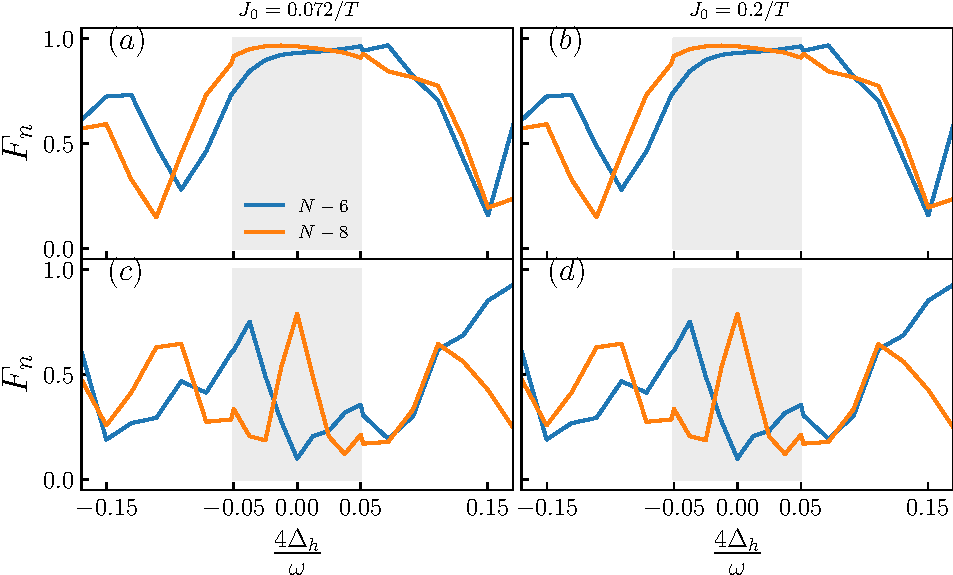
\includegraphics[width=10cm]{./figs/figure14.pdf}
				\end{center}
				\caption{Fidelity is plotted against several deviation values $\frac{4\Delta_h}{\omega}$ for different system size (N) for around CDT/DL point(top a,b-panels) and at away from CDT/DL point(bottom c,d-panels). The drive frequency is considered a constant $\omega 20$ value and the deviation in amplitude ($\Delta_h$) is added to h. Weak (a,c -panel) and strong (b,d-panel) are considered. The fidelity is found to be enough large around CDT/DL point (gray-colored region) in the top panels for both of the weak and strong coupling.}
				\label{Fig:aroundCDT}
			\end{figure}
			We found that $F_n$ is sufficiently large ($>0.85$) around the CDT/DL point for both of the spin coupling strengths. We have revised the manuscript at section 4.4 by replacing the sentence ``...even if there is a minor devation..." with ``... at significant deviation..." at page no.20,line no. 403. Additionally we have discussed this issue at Appendix-C at page no.28. 
			}
		\end{enumerate}
	
		\item The referee comments on, \comment{``\underline{DTC phase stability and entanglement entropy:}"}
		\begin{enumerate}
			\item \comment{``The paper seems to be intended for an audience from DTC and MBL/DMBL fields. However, for broader accessibility and comprehension, a brief introductory paragraph about realization and fundamental aspects of DTC within DMBL
			systems would be beneficial. How is DTC defined in these systems, and what are its fundamental properties? Additionally, how is $\omega$ chosen in relation to the periodicity of the Hamiltonian? Moreover, a preliminary explanation of how analyzing the time evolution of local magnetization and its FFT contributes to defining DTC would greatly enhance reader comprehension."}\\
		
			\response{ plan to write at the last ... 
			}
			\item \comment{``It is important to clarify the results shown in Fig. 7, where the behavior of regional magnetization might confuse new readers in the DTC field. This figure suggests that regional magnetization decreases over time under strong coupling and all-to-all interactions, which at the first glance seems to contradict the main text’s assertion that these conditions correspond to stable chimera states. Therefore, a comment  explaining how the magnetization relates to FFT based on the results would be helpful for correctly understanding the results."}\\
			
			\response{
			We thank the referee for the comment. In the figure the reginal magnetization for all-to-all interaction and strong coupling  decreases over time upto very large time 2000T in figure(9) in revised manuscript. In the earlier sections and results depicts that all-to-all interaction is the best suitable choice of spin interaction range for a stable chimeralike order and these results were based on finite large time upto 80T.
			
			In the FFT plot corresponding to the $M^z_A$ results are for very large time upto 2000T. The most dominant frequency is 0.5. However there are other frequencies exist in the FFT spectrum although their dominance (depends on second power of corresponding amplitude) is weaker than $\Omega/\omega=0.5$. For all-to-all interaction range, there is almost no significant frequency available expect at $\Omega/\omega=0.5$ for weak coupling. This manifests a stable chimera even at 2000T. However in case of strong coupling, other frequencies contributing larger FFT amplitudes affect the dynamics due to  $\Omega/\omega=0.5$. This contrasts the stability of chimeralike order in between  weak and strong coupling for the system of finite size N=8.
			
			\begin{figure}[h!]
				%\begin{center}
					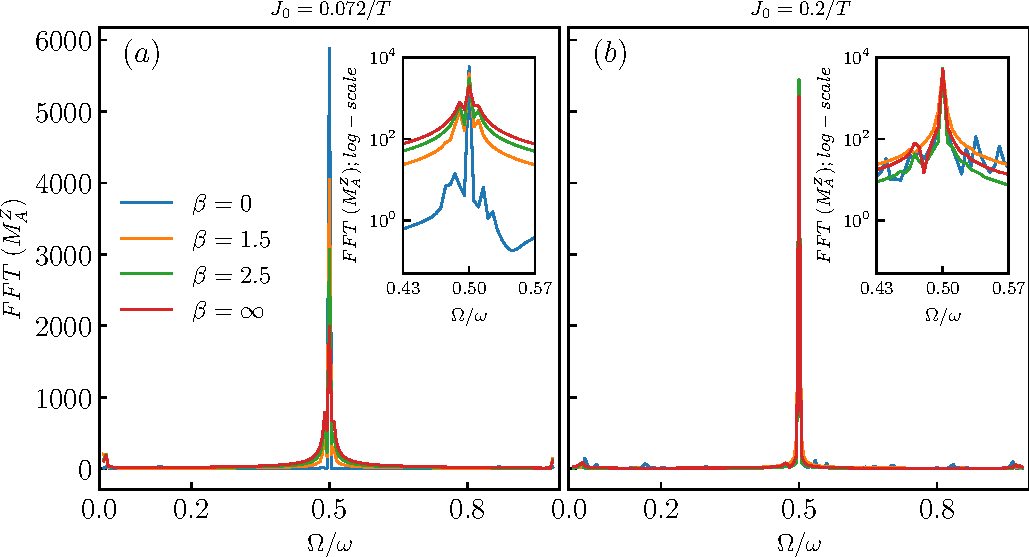
\includegraphics[width=10cm]{./figs/figure10.pdf}
				%\end{center}
				\caption{FFT for regonal magnetization ($M^z_A$) data obtained for time upto 2000T in region A. Weak(a-panel) and Strong (b-panel) is considered for several spin interaction ranges (defined by $\beta$) configuring the drive parameters at CDT/DL point. FFT is plotted also in log-scale plot in the inset of each panel for small frequency window to look closely into presence of frequencies is the temporal variation in $M^z_A$.}
				\label{Fig:aroundCDT}
			\end{figure}
			}
			We have elaborated our discussion on decrease in stability at strong coupling in the revised manuscript at page 17 and updated the FFT plot (figure 10 in revised manuscript) containing log-scale plot as inset figure and natural scale plot as the primary figure for better comprehension of the readers.
			\item \comment{``There appears to be inconsistency in the analysis of EE and regional magnetisation along with FFT. EE is shown for almost two times longer dynamics that regional magnetization and FFT. Could the authors provide a comparison of regional  magnetization and its FFT for the extended time frames considered for entanglement entropy?"}\\
			
			\response{We thank the referee for pointing out the mistake. We have extended our numerical simulation for regional magnetization and corresponding FFT upto 2000T in order to keep consistency in analysis of EE and regional magnetization. We have updated figures(9) $\&$(10) in the revised manuscript.
			}
		\end{enumerate}
		\item The referee comments on, \comment{``\underline{Applications of chimera state:} The introduction of Section 4 briefly touches upon applications of chimera states, but it lacks depth. How can the chimera state findings be applied in practice? Expanding on potential applications and providing references to existing literature will be beneficial. This would enrich the discussion and highlight the practical relevance of their findings."}
		
		\response{ MR : Akitada,  please write here... }
	\end{enumerate}

	\item[] {\bf Minor Comments}
	\begin{enumerate}
		\item The referee says, \comment{``\underline{Page 6, lines 30-31 and page 18, lines 47-48:} please add a reference to the Baker-Campbell-Hausdorff formula, e.g. [67] as in the Appendix B, page 22, lines 44-45"}\\
		
		\response{We thank the referee for poiting out the mistake. We have included reference to Baker-Campbell-Hausdorff formula at the suggested page 6.}
		\item The referee says, \comment{``\underline{Page 6, lines 46-48:} clarify what is $\mathcal{J}_0$, e.g. “of the higher roots of zeroth-order Bessel function $\mathcal{J}_0$”"}\\
		
		\response{We thank the referee for the comment. The analytical result suggest that at any one of the roots of Bessel function $\mathcal{J}_0\left(\frac{4h}{\omega}\right)$ results in nullify the dynamics due to $\hat{H}_2$ which manifests dynamical localization. 
		We have corrected the manuscript by eleminating the ``higher" word.
		\item The referee comments on, \comment{``\underline{Page 8, caption of Fig. 3:}"}}
		\begin{enumerate}
			\item The referee says, \comment{``refine the caption for clarity: “plotted for different values of amplitude h of the periodic drive. The x-coordinate plots 4h/$\omega$, where drive frequency is kept constant $\omega$=20..."}\\
			
			\response{We thank the referee for the comment. We have modified the sentence in revided manuscript to ``The quasi-energies are plotted for different values of $h,\omega$, the amplitude, and frequency of the periodic drive, respectively'' in order to maintain clarity in content in manuscript.}\\
			
			\item The referee says, \comment{``The first such point is shown...” $\rightarrow$ “The first two points are shown..."}
			
			\response{We gratefully thank the referee for the comment and suggestion. We have modified the sentence in the revised manuscript according to the suggestion of the referee.}
		\end{enumerate}
	
		\item The referee comments on, \comment{``\underline{Page 9, caption of Fig. 4:}"}
		\begin{enumerate}
			\item The referee says, \comment{``This is the suggestion of a notation change for smoother reading: “Site(i)” → “i”, 
			e.g. “for each i-th spin at region A (i=0,1,2,3) and region B (i=4,5,6,7)...”. To implement this modification consistently: change the x-coordinate labels in the Fig. 4 from “Site(i)” → “i”, and update accordingly the main text/ figures/ captions to
			maintain consistency"}\\
		
			\response{We thank the referee for the suggestion. We have modified the caption and figures by replacing ``Site(i)” → ``i” through out the manuscript.}
			\item The referee says, \comment{``Revise “spin coupling ($J_0$=0.027/T)” $\rightarrow$ “spin coupling ($J_0$=0.072/T)”}\\
			
			\response{We thank the referee for pointing out the typographical error. We have corrected it to ``($J_0$=0.072/T)" in the revised manuscript.}\\
			\item The referee says, \comment{``Please add also the information for which root of the Bessel function the plot is obtained."}\\
			
			\response{We thank the referee for the comment. We have selected the first root of Bessel function $\mathcal{J}_0\left(\frac{4h}{\omega}\right)$ to define the CDT/DL point for all numerical simulation and analytical consideration. We have corrected it in the revised manuscript by mentioning the selection of the first root of Bessel function $\mathcal{J}_0\left(\frac{4h}{\omega}\right)$ in the caption of figure 4.}
		\end{enumerate}
		\item The referee comments on, \comment{``\underline{Page 10, Fig. 5:}"}
		\begin{enumerate}
			\item The referee says, \comment{``Define $M_A^z$, which appears in the y-label, in the main text or the caption for
			clarity. The formal introduction of regional magnetization occurs in Section 4, while Fig. 5 is situated within Section 3."}\\
		
			\response{We thank the referee for pointing out the mistake. We had labeled the figure 5 y-coordinate incorrectly. The figure 5 presents FFT analysis on the local magnetization numerical data of a selected site i=1 in region A. We have corrected and updated the figure 5 in revised manuscript with FFT linear-scale data in primary figure and corresponding log-scale data in set figure.}\\
			\item The referee says, \comment{``Specify a CDT/DL point, i.e. to which root of the Bessel function it corresponds"}\\
			
			\response{We thank the referee for the comment. We have considered the first root of $\mathcal{J}_0\left(\frac{4h}{\omega}\right)$ as the CDT/DL point and we have this selection of CDT/DL point consistent thorugh out in the revised manuscript.}\\
		\end{enumerate}
		\item The referee comments on, \comment{``\underline{Page 11, lines 50-51:} Specify “a CDT/DL point...” while throughout the paper the root of the Bessel function is changing, e.g. Fig. 4 and Fig. 5"}\\
		
		\response{We thank the referee for the comment. We have considered the first root of $\mathcal{J}_0\left(\frac{4h}{\omega}\right)$ as the CDT/DL point and we have this selection of CDT/DL point consistent thorugh out in the revised manuscript.}\\
		
		\item The referee comments on, \comment{``\underline{Page 13, Fig 8:} Correct the notation “$\omega/\omega_D$” → “$\Omega/\omega$”"}\\
		
		\response{We thank the referee to point out the typographical error. We have corrected “$\omega/\omega_D$” → “$\Omega/\omega$” in the caption of the respective figure the revised manuscript.}
		\item The referee says, \comment{``Ensure all paper captions are reviewed for consistency. Additionally, include all relevant
			parameters in the captions that would enable interested readers to reproduce your
			results effectively."}\\
		
		\response{We thank the referee for the comment and kind suggestion. We have gone through the entire manuscript and tried to maintain consistency in the parameters and notations. We expect  better comprehension and feasibility in reproduction of all the findings we present in this paper.}
	\end{enumerate}

	\newpage
	\noindent \textbf{Response to the Referee: 3's comment}
	\begin{enumerate}
		\item The referee says, \comment{``My main concern is regarding the context in which the word “chimera” has been used
			in this work. The word chimera was originally used for the co-existence of synchronized and unsynchronized dynamics of coupled “identical” oscillators in the “Phys. Rev. Lett. 93, 174102 (2004)” which was initially discovered in the following
			works “Y. Kuramoto and D. Battogtokh, Nonlinear Phenom. Complex Syst. 5, 380 (2002), S. I. Shima and Y. Kuramoto, Phys. Rev. E 69, 036213 (2004)”. The surprise that led to the discovery of the chimera state resided in the fact that all the
			subsystems were identical and were subjected to the same environment but behaved differently only due to different initial configurations. But in this and the earlier work mentioned by authors “Phys. Rev. Lett. 126, 120606 (2021)”, regions A and B are under different drive conditions. Hence, the spins in these regions are not under identical environments. In such a configuration, it is trivial that both regions can behave differently since they are subjected to different drive conditions. Hence, this co-existence of different phases under inhomogeneous drive conditions for different
			regions does not fall under the novel phenomenon of “chimera”.\\
			
			I understand that this issue arises due to the fact that the related work “Phys. Rev. Lett. 126, 120606 (2021)” has referred to this phenomenon as a “chimera state”, even though one of the authors from the same paper has used the definition of the identical oscillator in their earlier work “Phys. Rev. E 92, 062924 (2015)”. Therefore, I request the authors either remove the word chimera completely or use the word “chimeralike state” which has been used in the work “Phys. Rev. E 103, 012214 (2021)” where authors have discovered a chimeralike state in almost-identical oscillators. Along with this, authors should provide a clear distinction that the definition of “chimeralike state” used in this work differs from the definition involving identical oscillators and follows from the earlier work “Phys. Rev. Lett. 126, 120606 (2021)” and “Phys. Rev. E 103, 012214” which involve non-identical systems. I
			suppose this is crucial to avoid misunderstandings and further confusion about the novel “Chimera State” for the readers of this reputed journal."}\\
		
			\response{We thank the referee for the comment and suggestion. We agree with the referee that the proposed chimera state in quantum spin-1/2 system is distinct from the classical chimera in systems of identical oscillators. The proposed quantum model experiences two non-homogeneous Hamiltonian which contradicts with basic criterion for generic classical chimera phenomena where ther identical oscillators undergoes similar enviornment. However quantum mechanics follows the Schr\"{o}dinger dynamics which is linear while classical dynamics can be non-linear. Therefore one can not expect similar emergent phenomena in qunautm mechanics in comparision to classical phenomena. This raises concerns in naming such a novel phenomena `chimera' in our proposed quantum system. We thank the referee for suggestion to modify the `chimera state' term to `chimeralike state'. We agree with the referee and modified each and every `chimera state' word to `chimeralike state' or `chimeralike order' through out the revised manuscript as well as in the article title.}
		
		\item The referee says, \comment{``Adding to the previous point on chimera-like states, it would be interesting to see if the chimera state emerges even for almost the same drive conditions for regions A and B, i.e. for $\epsilon A \approx \epsilon B$ where they only differ by a small value."}\\
		
		\response{We thank the referee for this comment. We have extended our investigation for the cases when spin rotational errors $\epsilon_A,B$ are close enough to be $\epsilon A \approx \epsilon B$. We have numerically calculated the regional magnetization and plotted for several values maintaining $\epsilon A \approx \epsilon B$ for different spin interaction ranges and plotted in figure 8 in the revised manuscript.
		We found that the small values $\epsilon A \approx \epsilon B$ the spins in the both of the region A and B exhibits time crystalline behavior however in course of time DTC phase melts. With gradual increase in $\epsilon A \approx \epsilon B$ we observe the emergence of DMBL phase in both of the regions. Thus a stable DTC-DMBL chimeralike order can not occur in the condition when $\epsilon A \approx \epsilon B$.} \\
	
		\item The referee says, \comment{``Authors can also investigate the onset of the chimera state as a function of $\epsilon A$ - $\epsilon B$."}\\
		\response{We thank the referee for the comment. We have considered a large number of $\epsilon_A$ and $\epsilon_B$ in order to investigate the dependence of stability of the DTC-DMBL chimeralike order and numerically calculated regional magnetization and plotted in figure 8. In the figure we have considered a small value of $\epsilon_A$ and then varied $\epsilon_B$ and vice versa. We observe that when $\epsilon A$ - $\epsilon B$ is minimum $~\sim -1.0$ the DTC in region A and DMBL in region B is most stable as can be observed in panel-a in figure 8. It is intriguing that we   $\epsilon A$ - $\epsilon B$ is maximum $~\sim +1.0$ a stable DTC can be found inregion B and a subtle DMBL is found in region A. This concluded that at the extremum values of  $\epsilon A$ - $\epsilon B$, a stable DTC-DMBL chimera like order is . Also varying $\epsilon A$ - $\epsilon B$ values regional selection over phases can be controlled. We have discussed it in revised manuscript from page 14 to 16, section 4.1 Regional magnetization. }
		
		\item The referee says, \comment{``To avoid confusion, the 45th line of Page 2 should be modified to indicate that the concept of “time crystal” was introduced by Frank Wilczek, not just the Discrete time crystals."}\\
		
		\response{We thank the referee for pointing out the mistake. We have corrected and modified the sentece from `` The concept was
		first proposed by Frank Wilczek " to ``The time crystal (TC) was first proposed by Frank Wilczek \dots" in the revised manuscript.}
	
		\item The referee says, \comment{``$J_0$ is not defined after equation 7 in the main text."}\\
		
		\response{We thank the referee for pointing out the typographical mistake. We have replaces $\mathcal{J}_0$ with $\mathcal{J}_0\left(\frac{4h}{\omega}\right)$. in the revised manuscript.}
		
		\item The referee says, \comment{``Recent works have not been included in the manuscript, I list some of the recent work on chimera states in time crystals and observation of discrete-time crystals for the consideration of authors:."}
		\begin{enumerate}
			\item \comment{``Observation of a Dissipative Time Crystal”, Phys. Rev. Lett. 127, 043602 (2021)"}
			\item \comment{``Observation of a Prethermal U(1) Discrete Time Crystal”, Phys. Rev. X 13, 041016 (2023)"}
			\item \comment{``Observation of time crystal comb in a driven-dissipative system”, arXiv:2402.13112 (2024)}
			\item \comment{``Exotic synchronization in continuous time crystals outside the symmetric subspace”, arXiv:2401.00675 (2024)"}
		\end{enumerate}
	\end{enumerate}
\end{enumerate}
		
		

	
	
\noindent \textbf{Summary of important changes to the  manuscript}
\begin{enumerate}
	\item write the changes you have made$\dots$.
\end{enumerate}
\end{document}